\section{Appendix}
\label{sec:appendix}

\subsection{Links}
\label{sec:appendix:links}

\subsubsection{Google Drive Link}
\label{sec:appenfix:links:gdrive}
\begin{enumerate}
    \item \url{https://drive.google.com/open?id=1xhN2p1EFsN0P4SPehv_dIEZSN-SREN-n}
    \item \url{http://bit.ly/2PBo3DU} 
\end{enumerate}

\subsubsection{Bitbucket Link (No Data)}
\label{sec:appenfix:links:bitbucket}
\begin{enumerate}
    \item \url{https://bitbucket.org/Ajg2/ml_cw1/src/master/}
    \item \url{http://bit.ly/ML\_source} 
\end{enumerate}


\FloatBarrier
\subsection{Classifier Settings}
\label{sec:appendix:classifier}


\FloatBarrier
\subsubsection{Random Forest User Classifier Settings}
\label{sec:appendix:classifier:rfucs}

\begin{figure}[!htb]
	\centering
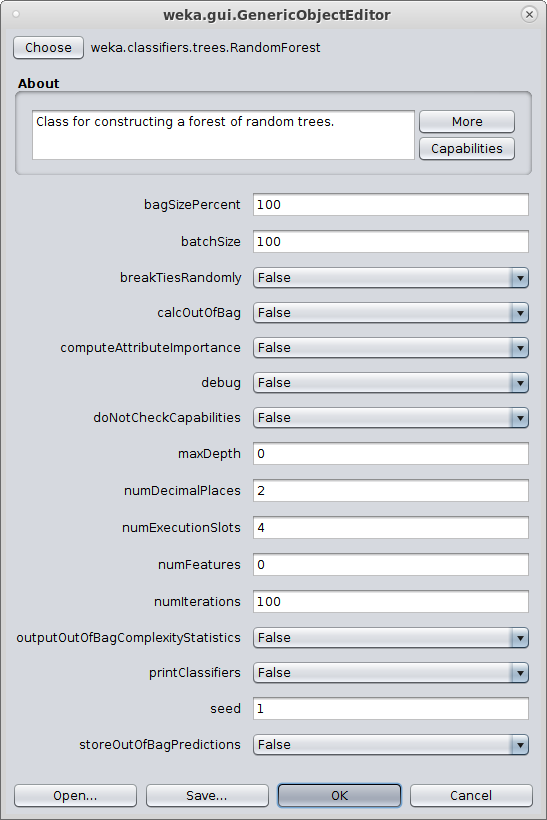
\includegraphics[width=0.6\textwidth]{imgs/userClassifier/noSplit/all/Train-and-Test/tree_classifier.png} \\
	\caption{Semi-Manual Tree's Random Forrest Classifier Settings}
	\label{fig:appendix:classifier:rfucs}
\end{figure}


\FloatBarrier
\subsection{Charts and Tables}
\label{sec:appendix:charts_tables}

\FloatBarrier
\subsubsection{Random Forest Results}
Below is a summary of the experiments I ran using Random Forest
\begin{figure}[hbt!]
	\centering
      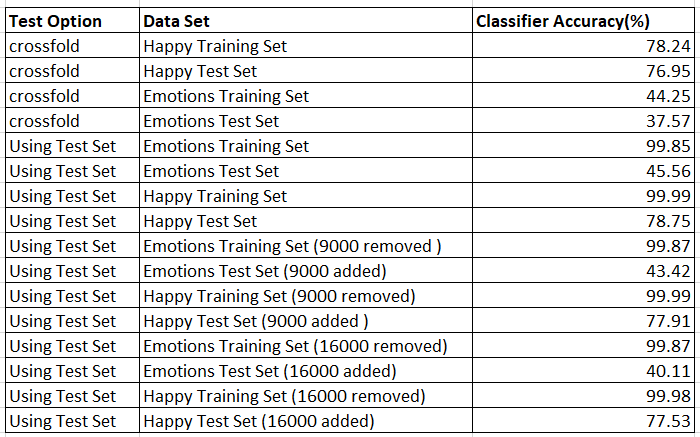
\includegraphics[width=\textwidth]{imgs/RandomForest/RandomForest_Main.png} \\
	\caption{Default settings, on the various testing options}
	\label{fig:randomforest_main}
\end{figure}

\begin{figure}[hbt!]
	\centering
      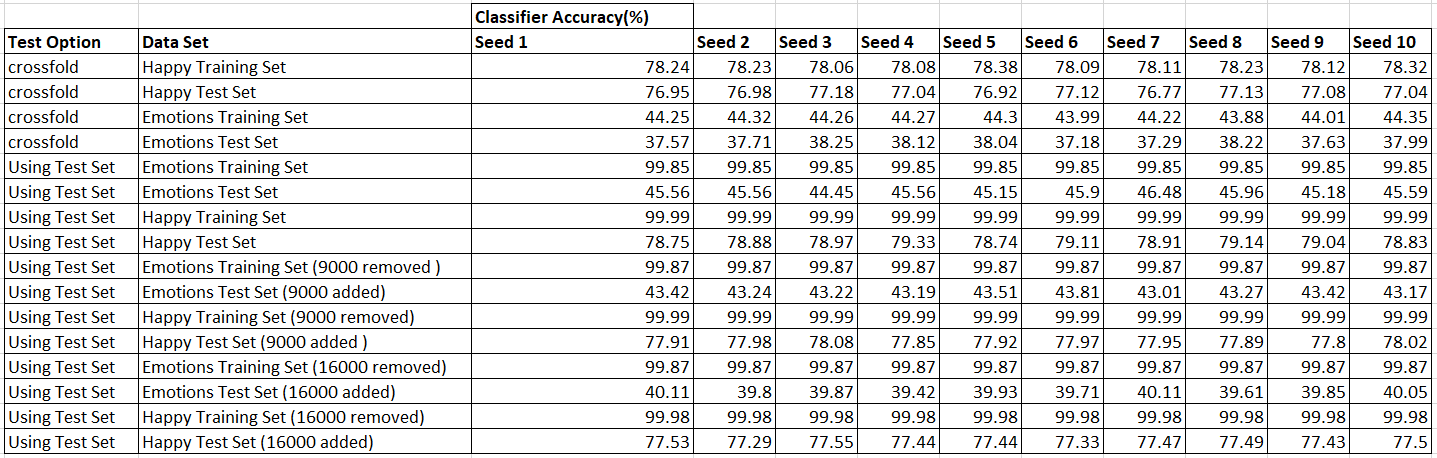
\includegraphics[width=\textwidth]{imgs/RandomForest/RandomForest_Seed.png} \\
	\caption{Changing seed setting, on the various testing options}
	\label{fig:randomforest_seed}
\end{figure}
\begin{figure}[hbt!]
	\centering
      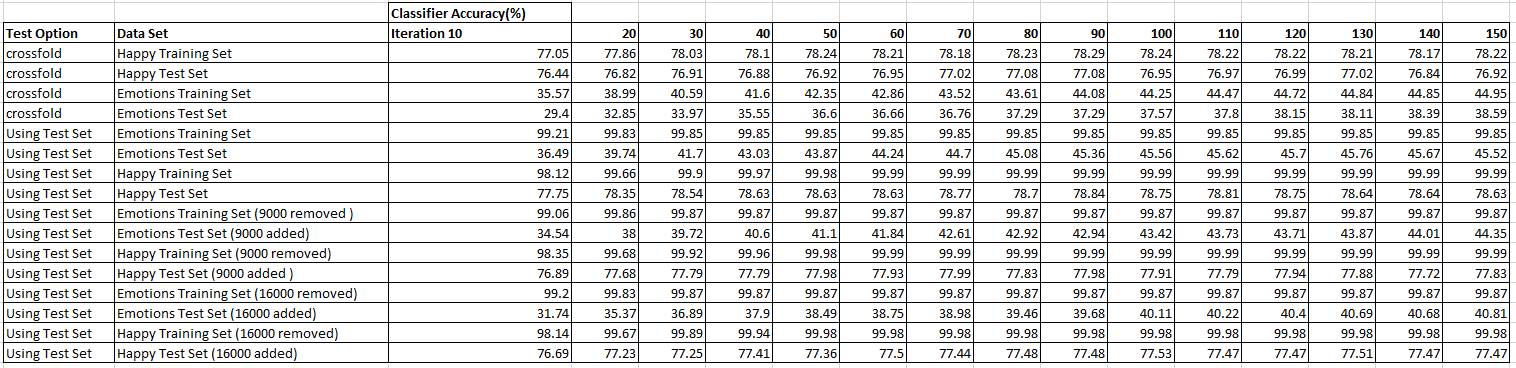
\includegraphics[width=\textwidth ,height=5cm]{imgs/RandomForest/RandomForest_Iteration.png} \\
	\caption{Changing iteration setting, on the various testing options}
	\label{fig:randomforest_iteration}
\end{figure}

\begin{figure}[hbt!]
	\centering
      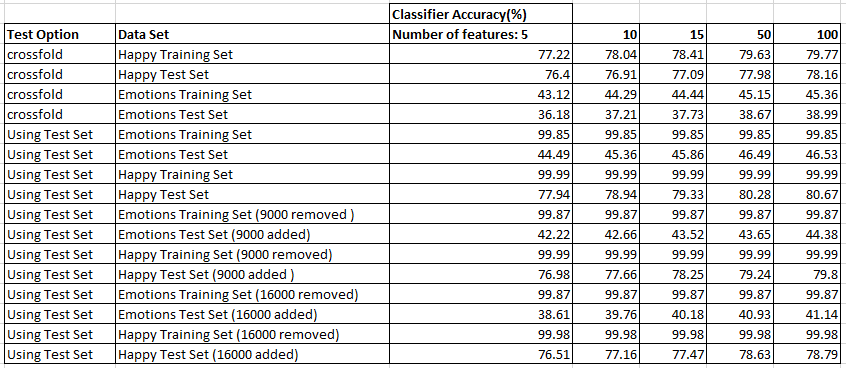
\includegraphics[width=\textwidth]{imgs/RandomForest/RandomForest_NumOfFeatures.png} \\
	\caption{Changing number of features setting, on the various testing options}
	\label{fig:randomforest_numfeatures}
\end{figure}

\begin{figure}[hbt!]
	\centering
      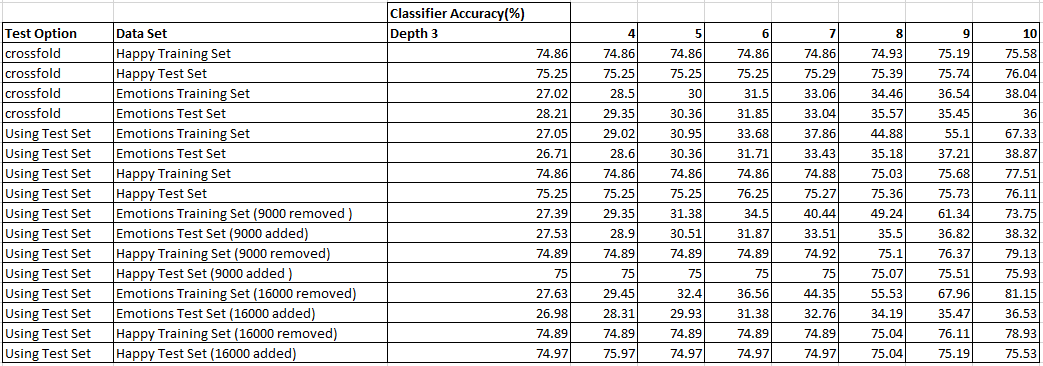
\includegraphics[width=\textwidth]{imgs/RandomForest/RandomForest_Depth.png} \\
	\caption{Changing depth setting, on the various testing options}
	\label{fig:randomforest_numfeatures}
\end{figure}


